\documentclass[10pt]{article}
\usepackage[verbose, a4paper, hmargin=2.5cm, vmargin=2.5cm]{geometry}

\usepackage{fontspec}
\usepackage{ctex}
\usepackage{paratype}

\usepackage{amsmath}
\usepackage{amssymb}
\usepackage{amsfonts}
\usepackage{esint}
\usepackage{stmaryrd}

\usepackage[mathbf=sym]{unicode-math}
\setmainfont{STIX Two Text}
\setmathfont{STIX Two Math}

\setsansfont{Arial}
\setmonofont{Courier New}

\usepackage{makecell}
\usepackage{wasysym}
\usepackage{pifont}
\usepackage[export]{adjustbox}
\usepackage{graphicx}
\usepackage{mdframed}
\usepackage{booktabs,array,multirow}
\usepackage{tabularx}
\usepackage{hyperref}
\hypersetup{colorlinks=true, linkcolor=blue, filecolor=magenta, urlcolor=cyan,}
\urlstyle{same}
\usepackage[most]{tcolorbox}
\definecolor{mygray}{RGB}{240,240,240}
\tcbset{
  colback=mygray,
  boxrule=0pt,
}
\usepackage{tikz}

% 定义留白命令 - 用于教师板书
\newcommand{\boardspace}[1]{%
  \par\vspace{#1}
}

% 定义中难题留白（大幅留白供教师板书）
\newcommand{\hardboardspace}{%
  \par\vspace{5cm}
  \hfill\textit{（此处留白供课堂讲解）}
  \par\vspace{1cm}
}

% 定义大题留白
\newcommand{\largeboardspace}{%
  \par\vspace{8cm}
  \hfill\textit{（此处留白供课堂讲解与板书推导）}
  \par\vspace{1cm}
}

\graphicspath{ {./images/} }
\newcommand{\HRule}{\begin{center}\rule{0.9\linewidth}{0.2mm}\end{center}}
\newcommand{\customfootnote}[1]{
  \let\thefootnote\relax\footnotetext{#1}
}
\newcommand{\lt}{\mathrel{<}}
\newcommand{\gt}{\mathrel{>}}
\newcommand*\circled[1]{\tikz[baseline=(char.base)]{\node[shape=circle,draw,inner sep=1.5pt] (char) {\small #1};}}
\setcounter{MaxMatrixCols}{256}
\begin{document}
\begin{center}
\Large\textbf{2026届崇明区高三下二模数学试卷}\\[0.5em]
\normalsize\textit{（学生版·课堂使用）}
\end{center}

\section*{一、填空题（第1-9题每题4分，第10-12题每题5分，共51分）}

1. 集合 \(A = \{ 2,4,6,8,{10}\} ,B = \left( {-1,6}\right)\) ，则 \(A \cap  B =\) \_\_\_\_\_.

\boardspace{1.5cm}

2. 不等式 \(\left| {x - 1}\right|  < 2\) 的解为\_\_\_\_.

\boardspace{1.5cm}

3. 若复数 \(z\) 满足 \(\frac{z}{1 + \mathrm{i}} = \mathrm{i}\) ( \(\mathrm{i}\) 为虚数单位),则 \(z =\) \_\_\_\_.

\boardspace{1.5cm}

4. 已知向量 \(\overrightarrow{a} = \left( {k,2}\right)\) ， \(\overrightarrow{b} = \left( {2,1}\right)\) ，若 \(\overrightarrow{a}\bot \overrightarrow{b}\) ，则实数 \(k =\) \_\_\_\_.

\boardspace{1.5cm}

5. 若 \(x > 0,y > 0\) ，且 \({xy} = 1\) ，则 \(x + {2y}\) 的最小值为\_\_\_\_.

\boardspace{1.5cm}

6. 已知 \(\cos \theta  =  - \frac{3}{5}\) ，则 \(\cos {2\theta }\) 的值为\_\_\_\_.

\boardspace{1.5cm}

7. 从一副去掉大小王的 52 张扑克牌中随机抽取一张牌,事件 \(A\) 表示 ``取得的牌面是 \(A\) '',事件 \(B\) 表示``取得的牌的花色是黑桃''，则 \(P\left( {B \mid  A}\right)\) 为\_\_\_\_.

\boardspace{1.5cm}

8. 在 \(\bigtriangleup  {ABC}\) 中，角 \(A\) 、 \(B\) 、 \(C\) 所对的边长分别为 \(a\) 、 \(b\) 、 \(c\) . 若 \(A = {45}^{ \circ  }\) ， \(C = {30}^{ \circ  }\) ， \(c = \sqrt{2}\) ，则 \(a =\) \_\_\_\_.

\boardspace{1.5cm}

9. 已知 \({\left( x - 1\right) }^{3} + {\left( x + 1\right) }^{4} = {x}^{4} + {a}_{1}{x}^{3} + {a}_{2}{x}^{2} + {a}_{3}x + {a}_{4}\) ,则 \({a}_{1} =\) \_\_\_\_.

\boardspace{1.5cm}

% 第10题开始为中难题，留足留白
10. 如图,已知圆柱的一个截面边界是椭圆 \(\Gamma\) ,其中 \(\Gamma\) 的长轴 \({AC}\) 为该圆柱轴截面的对角线,短轴长等于圆柱底面直径的长. 将圆柱侧面沿母线 \({AB}\) 展开,则椭圆 \(\Gamma\) 在展开图中恰好为一个周期的三角函数图像. 若该段曲线是函数 \(y = 1 - \sqrt{3}\sin \frac{x}{2}\) 的图像的一部分,则椭圆 \(\Gamma\) 的离心率为\_\_\_\_.

\begin{center}
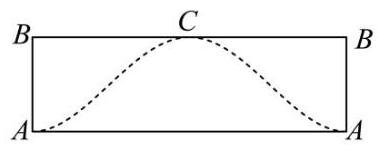
\includegraphics[max width=0.3\textwidth]{images/bo_d7ffhcs91nqc73erb3p0_1_1116_1751_378_152_0.jpg}
\end{center}

\hardboardspace

11. 设 \({f}_{1}\left( x\right)  = \sin x,{f}_{2}\left( x\right)  = \cos \left( {x + \frac{\pi }{6}}\right)\) . 若对任意 \(t \in  \mathbf{R}\) ,存在 \(i \in  \{ 1,2\}\) 使得函数 \(y = {f}_{i}\left( x\right)\) 在区间 \(\left\lbrack  {t,t + a}\right\rbrack  \left( {a > 0}\right)\) 上是单调函数，则实数 \(a\) 的取值范围是\_\_\_\_.

\hardboardspace

12. 已知首项为 1 的等比数列 \(\left\{  {a}_{n}\right\}\) 满足对任意的正整数 \(m,n\) 都有 \(\left| {{a}_{m} - {a}_{n}}\right|  \leq  \frac{1}{3}\left| {m - n}\right|\) ,则等比数列 \(\left\{  {a}_{n}\right\}\) 的公比 \(q\) 的取值范围是\_\_\_\_.

\hardboardspace

\section*{二、单选题（每题5分，共20分）}

13. 在空间内, 异面直线所成角的取值范围是( )

A. \(\left( {0,\frac{\pi }{2}}\right)\) B. \(\left( {0,\frac{\pi }{2}}\right\rbrack\) C. \(\left\lbrack  {0,\frac{\pi }{2}}\right)\) D. \(\left\lbrack  {0,\frac{\pi }{2}}\right\rbrack\)

\boardspace{2cm}

14. 下列函数中,在 \(\mathbf{R}\) 上为严格增函数的是( )

A. \(y = {x}^{2}\) B. \(y = \left| x\right|\) C. \(y = \sin x\) D. \(y = {x}^{3}\)

\boardspace{2cm}

15. 已知 \(A\left( {-a,0}\right) ,B\left( {a,0}\right) ,{l}_{1} : {ax} - y = 0,{l}_{2} : {ax} + y = 0\) ,其中 \(a > 1\) ,点 \(P\) 为平面内一点,记点 \(P\) 到 \({l}_{1}\) , \({l}_{2}\) 的距离分别为 \({d}_{1},{d}_{2}\) ,则下列条件中能使点 \(P\) 的轨迹为椭圆的是 ( )

A. \(\left| {PA}\right|  + \left| {PB}\right|  = {2a}\) B. \({\left| PA\right| }^{2} + {\left| PB\right| }^{2} = 4{a}^{2}\)

C. \({d}_{1}^{2} + {d}_{2}^{2} = 4{a}^{2}\) D. \({d}_{1} + {d}_{2} = {4a}\)

\hardboardspace

16. 已知函数 \(y = f\left( x\right) ,x \in  \mathbf{R}\) . 定义集合 \(M = \left\{  {{x}_{0} \mid  \text{ 对任意的 }x > {x}_{0}\text{ ,都有 }f\left( x\right)  \leq  f\left( {x}_{0}\right) }\right\}\) . 对于所有使得 \(M = \left\lbrack  {-1,2}\right\rbrack\) 的函数 \(y = f\left( x\right)\) ,有以下两个命题:  \circled{1} 存在函数 \(y = f\left( x\right)\) 在 \(x =  - 2\) 处取极小值;  \circled{2} 存在函数 \(y = f\left( x\right)\) 图像是连续曲线. 下列判断正确的是( )

A.  \circled{1}  \circled{2} 都真 B.  \circled{1} 真\circled{2} 假 C.  \circled{1} 假\circled{2} 真 D.  \circled{1}  \circled{2} 都假

\hardboardspace

\section*{三、解答题（共79分）}

17. （14分）如图，在直三棱柱 \({ABC} - {A}_{1}{B}_{1}{C}_{1}\) 中， \({AB} = {BC} = \sqrt{2},{AC} = {A{A}_{1}} = 2\) ，且 \(D,E\) 分别是 \({AC},{A}_{1}{C}_{1}\) 的中点.

\begin{center}
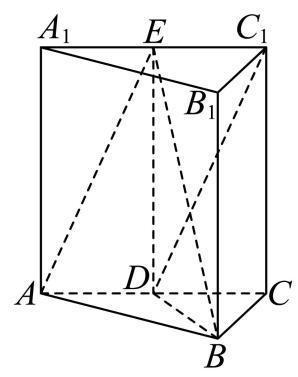
\includegraphics[max width=0.25\textwidth]{images/bo_d7ffhcs91nqc73erb3p0_5_1200_1616_298_377_0.jpg}
\end{center}

(1)证明: \(D{C}_{1}//\) 平面 \({ABE}\) ；

(2)求三棱锥 \({C}_{1} - {ABE}\) 的体积.

\largeboardspace

\newpage

18. （14分）2025 年 11 月, 教育部等五部门联合印发《关于实施学生体质强健计划的意见》, 明确要求``中小学生每天综合体育活动时间不少于 2 小时''. 某学校为了解政策落实情况及其对学生视力的影响，随机抽取了 100 名学生进行每周累计体育活动时长的调查, 得到如下频率分布表:

\begin{center}
\adjustbox{max width=\textwidth}{
\begin{tabular}{|c|c|c|c|c|c|}
\hline
每周活动总时长 (单位:时) & \(\lbrack 0,7)\) & \(\lbrack 7,{14})\) & \(\lbrack {14},{21})\) & \(\lbrack {21},{28})\) & [28,35] \\
\cline{1-6}
频率 & 0.15 & 0.25 & 0.35 & 0.15 & 0.1 \\
\cline{1-6}
\hline
\end{tabular}
}
\end{center}

同时，对这 100 名学生的视力进行了检查，将视力达到 5.0 及以上定为``视力良好''，低于 5.0 定为``视力一般''，得到如下 \(2 \times  2\) 列联表 (部分数据缺失):

\begin{center}
\adjustbox{max width=\textwidth}{
\begin{tabular}{|c|c|c|c|}
\hline
\phantom{X} & 视力良好 & 视力一般 & 合计 \\
\cline{1-4}
活动时间达标 (不少于 14 小时) & 40 & \phantom{X} & \phantom{X} \\
\cline{1-4}
活动时间未达标 (低于 14 小时) & \phantom{X} & 30 & \phantom{X} \\
\cline{1-4}
合计 & \phantom{X} & \phantom{X} & 100 \\
\cline{1-4}
\hline
\end{tabular}
}
\end{center}

(1)从活动时长在 \(\left\lbrack  {0,7}\right)\) 和 \(\left\lbrack  {{28},{35}}\right\rbrack\) 的学生中，按比例分层随机抽样抽取 5 人进行座谈. 若从文 5 人中随机抽取 2 人，设 \(X\) 为抽取的 2 人中活动时长在 \(\left\lbrack  {{28},{35}}\right\rbrack\) 的人数，求 \(X\) 的分布列和数学期望 \(E\left\lbrack  X\right\rbrack\) ；

(2)依据 \(\alpha  = {0.05}\) 的独立性检验，判断是否有 95\%的把握认为``视力情况''与``体育活动时长是否达标''有关. 参考公式及数据:

\circled{1} \({\chi }^{2} = \frac{n{\left( ad - bc\right) }^{2}}{\left( {a + b}\right) \left( {c + d}\right) \left( {a + c}\right) \left( {b + d}\right) }\) ，其中 \(n = a + b + c + d\) .

\circled{2} \(P\left( {{\chi }^{2} \geq  {6.635}}\right)  \approx  {0.01}\) ， \(P\left( {{\chi }^{2} \geq  {5.024}}\right)  \approx  {0.025}\) ， \(P\left( {{\chi }^{2} \geq  {3.841}}\right)  \approx  {0.05}\) ， \(P\left( {{\chi }^{2} \geq  {2.706}}\right)  \approx  {0.1}\) .

\largeboardspace

\newpage

19. （14分）设函数 \(f\left( x\right)  = {x}^{2} - x + a\ln x,a \in  \mathbf{R}\) .

(1)若 \(a = 1\) ，求 \(f\left( x\right)\) 的图象在 \(x = 1\) 处的切线方程；

(2)若 \(f\left( x\right)  \geq  0\) 在 \(\lbrack 1, + \infty )\) 上恒成立，求 \(a\) 的取值范围；

\largeboardspace

\newpage

20. （18分）已知椭圆 \(C : \frac{{x}^{2}}{4} + \frac{{y}^{2}}{3} = 1\) .

(1)求椭圆 \(C\) 的离心率 \(e\) ；

(2)已知椭圆右顶点为 \(A\) ，设点 \(M\) 为 \(y\) 轴正半轴上一点，点 \(P\) 为椭圆 \(C\) 上的一点. 若 \(\overrightarrow{AP} = 2\overrightarrow{PM}\) ，求点 \(M\) 的坐标;

(3)已知 \(G\left( {\frac{5}{2},0}\right)\) ,过点 \(R\left( {4,0}\right)\) 的直线交椭圆 \(C\) 于 \(D,E\) 两点,直线 \({DG}\) 交直线 \(x = 1\) 于点 \(H\) ,证明: \({EH} \bot  y\) 轴.

\begin{center}
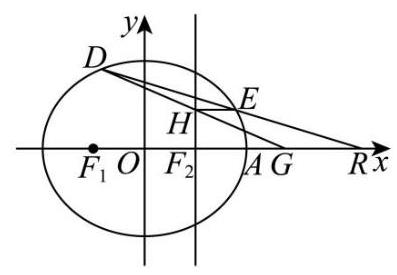
\includegraphics[max width=0.35\textwidth]{images/bo_d7ffhcs91nqc73erb3p0_9_1087_1636_397_275_0.jpg}
\end{center}

\largeboardspace

\newpage

21. （19分）函数 \(y = f\left( x\right) ,x \in  \mathbf{R}\) 是减函数,即对于任意的 \({x}_{1},{x}_{2} \in  \mathbf{R}\) ,当 \({x}_{1} < {x}_{2}\) 时,均有 \(f\left( {x}_{1}\right)  \geq  f\left( {x}_{2}\right)\) .

(1)若 \(f\left( x\right)  =  - {x}^{3} + {ax}\) ，求实数 \(a\) 的取值范围；

( 2 )是否存在函数 \(y = f\left( x\right)\) 是偶函数，且满足 \(f\left( {f\left( x\right) }\right)  = x\) 对所有 \(x \in  \mathbf{R}\) 成立？若存在，请举出一个满足条件的函数, 若不存在, 请说明理由;

(3) 设 \(g\left( x\right)  = \sin x\) ，已知函数 \(h\left( x\right)  = f\left( x\right)  + g\left( x\right)\) 是周期函数，求证: \(f\left( x\right)\) 为常值函数.

\largeboardspace

\vfill
\begin{center}
\textit{— 试卷结束 —}
\end{center}

\end{document}
